\documentclass[11pt,a4paper]{article}
\usepackage[T1]{fontenc}
\usepackage[utf8]{inputenc}
\usepackage{lmodern}
\usepackage{textcomp}
\usepackage[left=1.8cm,right=1.8cm,top=3.0cm,bottom=2.2cm,headheight=36pt,headsep=12pt]{geometry}
\usepackage{multicol}
\usepackage{xcolor}
\usepackage{fancyhdr}\usepackage{tikz}
\usepackage{graphicx}
\usepackage{array}
\usepackage{amsmath,amssymb}
\usepackage{setspace}
\usepackage{longtable}
\graphicspath{{../}}
\definecolor{ygreen}{RGB}{46,139,87}\definecolor{dgreen}{RGB}{28,90,56}
\renewcommand{\normalsize}{\fontsize{10.9}{13.4}\selectfont}
\renewcommand{\familydefault}{\rmdefault}
\setlength{\parindent}{0pt}
\setlength{\columnsep}{0.8cm}
\setlength{\columnseprule}{0.4pt}
\setlength{\multicolsep}{3pt plus 1pt minus 1pt}
\renewcommand{\textsubscript}[1]{\ensuremath{_{\text{\fontsize{8}{8}\selectfont #1}}}}
\renewcommand{\textsuperscript}[1]{\ensuremath{^{\text{\fontsize{8}{8}\selectfont #1}}}}
\newcommand{\qn}[1]{\textbf{\fontsize{11.5}{13}\selectfont #1}}
\newcommand{\qsep}{\par\vspace{13pt}}
\newcommand{\fwrule}{\par\vspace{5pt}\noindent\rule{\linewidth}{1.4pt}\par\vspace{7pt}}
\newsavebox{\fitb}
\newcommand{\fitbox}[1]{\sbox{\fitb}{#1}\ifdim\wd\fitb>\linewidth\resizebox{\linewidth}{!}{\usebox{\fitb}}\else\usebox{\fitb}\fi}
\newcommand{\diqqat}[1]{\par\smallskip\noindent\textbf{Diqqat!} #1\par\medskip}
\newcommand{\javob}{\par\nopagebreak[4]\smallskip\noindent\textbf{Javob:} \rule[-2pt]{7.5cm}{0.4pt}\par\smallskip\noindent\textbf{Diqqat!} Javobingizni javoblar varaqasiga ko`chirib yozing.\par\medskip}
\pagestyle{fancy}
\fancyhf{}
\renewcommand{\headrulewidth}{1.6pt}\renewcommand{\headrule}{{\color{ygreen}\hrule height 1.6pt width\headwidth}}
\newcommand{\hdrlogo}{
\begin{tikzpicture}[baseline=0pt]\fill[ygreen,rounded corners=3pt] (0,0) rectangle (0.95,0.95);\node[white,font=\fontsize{24}{26}\bfseries\selectfont] at (0.475,0.47){K};\node[anchor=west,font=\fontsize{16}{18}\bfseries\selectfont,text=dgreen] at (1.15,0.66){KIMYO};\node[anchor=west,font=\footnotesize\scshape,text=gray] at (1.15,0.2){Milliy sertifikat\ \ 2026};\end{tikzpicture}}
\newcommand{\hdrpill}[1]{\begin{tikzpicture}[baseline=0pt]\node[fill=ygreen,text=white,rounded corners=8pt,inner xsep=10pt,inner ysep=5pt,font=\fontsize{13}{15}\bfseries\selectfont] at (0,0.475){#1};\end{tikzpicture}}
\fancyhead[L]{\hdrlogo}
\fancyhead[R]{\hdrpill{11-variant}}

\fancyfoot[C]{\thepage}
\fancypagestyle{first}{\fancyhf{}\renewcommand{\headrulewidth}{1.6pt}\renewcommand{\headrule}{{\color{ygreen}\hrule height 1.6pt width\headwidth}}\fancyhead[L]{\hdrlogo}\fancyhead[R]{\hdrpill{11-variant}}\fancyfoot[C]{\thepage}}
\begin{document}
\normalsize
\thispagestyle{first}
\noindent\textit{Davriy jadvaldan foydalanish mumkin.}
\par\smallskip
\begin{multicols}{2}
\noindent\qn{1.} Quyidagilarni jism va moddalarga ajrating: alyuminiy, shakar, kislorod, qalam, stakan. Ulardan nechtasi modda?

\noindent A)~\textsl{4} \hfill B)~\textsl{2} \hfill C)~\textsl{3} \hfill D)~\textsl{5}\par
\qsep
\noindent\qn{2.} AgNO\textsubscript{3} ning suvli eritmasi inert elektrodlar bilan elektroliz qilinganda qaysi moddalar ajraladi?

\noindent\begin{tabular}{@{}p{0.47\linewidth}@{}p{0.47\linewidth}@{}}
A)~\textsl{Cu va Cl\textsubscript{2}} & B)~\textsl{Cu va O\textsubscript{2}} \\
C)~\textsl{H\textsubscript{2}, Cl\textsubscript{2} va NaOH} & D)~\textsl{Ag va O\textsubscript{2}} \\
\end{tabular}\par
\qsep
\noindent\qn{3.} Jadvalda nuklidlarning proton soni (\textit{Z}) va massa soni (A) berilgan:
\begin{center}
\renewcommand{\arraystretch}{1.15}
\fitbox{\begin{tabular}{|c|c|c|}\hline
\textbf{Nuklid} & \textbf{\textit{Z}} & \textbf{A} \\ \hline
\textit{X} & 20 & 40 \\ \hline
\textit{Y} & 20 & 42 \\ \hline
T & 21 & 40 \\ \hline
\textit{U} & 21 & 41 \\ \hline
\textit{V} & 20 & 42 \\ \hline
\end{tabular}}
\end{center}
\textit{X} nuklidning nechta izobari jadvalda keltirilgan?

\noindent A)~\textsl{1} \hfill B)~\textsl{2} \hfill C)~\textsl{3} \hfill D)~\textsl{4}\par
\qsep
\noindent\qn{4.} Quyidagi tuz eritmalari aralashtirilganda qaysilarida ham cho`kma, ham gaz hosil bo`ladi? 1) Al\textsubscript{2}(SO\textsubscript{4})\textsubscript{3} va Na\textsubscript{2}CO\textsubscript{3}; 2) FeCl\textsubscript{3} va Na\textsubscript{2}CO\textsubscript{3}; 3) CaCl\textsubscript{2} va Na\textsubscript{2}CO\textsubscript{3}; 4) Al\textsubscript{2}(SO\textsubscript{4})\textsubscript{3} va Na\textsubscript{2}S

\noindent A)~\textsl{1, 2} \hfill B)~\textsl{2, 3, 4} \hfill C)~\textsl{1, 3, 4} \hfill D)~\textsl{1, 2, 4}\par
\qsep
\noindent\qn{5.} Quyidagi moddalarning qaysilarida donor--akseptor bog` mavjud? 1) Cl\textsubscript{2}; 2) NaCl; 3) (NH\textsubscript{4})\textsubscript{2}SO\textsubscript{4}; 4) CO\textsubscript{2}

\noindent A)~\textsl{3} \hfill B)~\textsl{3, 4} \hfill C)~\textsl{2, 4} \hfill D)~\textsl{1, 2}\par
\qsep
\noindent\qn{6.} Nikel (\textit{Z} = 28) atomi elektron konfiguratsiyasida jami nechta juftlashgan elektron bor?

\noindent A)~\textsl{27} \hfill B)~\textsl{26} \hfill C)~\textsl{25} \hfill D)~\textsl{28}\par
\qsep
\noindent\qn{7.} SiO\textsubscript{2} tarkibida kremniy ning \textbf{valentligini aniqlang.}

\noindent A)~\textsl{\textit{V}} \hfill B)~\textsl{VII} \hfill C)~\textsl{VI} \hfill D)~\textsl{IV}\par
\qsep
\noindent\qn{8.} Radioaktiv izotopning boshlang`ich miqdorining 15/16 qismi parchalandi. Necha yarim yemirilish davri o`tgan?

\noindent A)~\textsl{5} \hfill B)~\textsl{3} \hfill C)~\textsl{8} \hfill D)~\textsl{4}\par
\qsep
\noindent\qn{9.} A elementi atomining ketma-ket ionlanish energiyalari diagrammada berilgan.
\begin{center}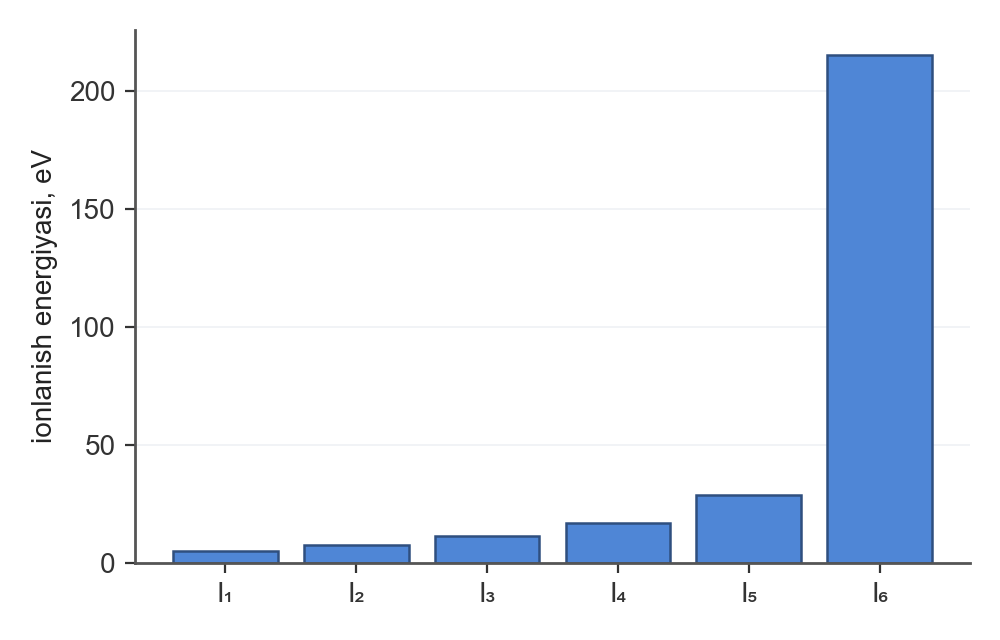
\includegraphics[width=0.86\linewidth]{rasmlar/gen/ie_v11_0.png}\end{center}
A elementining eng yuqori oksidi \textbf{formulasini toping.}

\noindent A)~\textsl{A\textsubscript{2}O} \hfill B)~\textsl{A\textsubscript{2}O\textsubscript{5}} \hfill C)~\textsl{AO} \hfill D)~\textsl{A\textsubscript{2}O\textsubscript{3}}\par
\qsep
\noindent\qn{10.} 16,8 g CaO va 8,1 g H\textsubscript{2}O aralashtirilib, reaksiya o`tkazildi. Hosil bo`lgan Ca(OH)\textsubscript{2} \textbf{massasini (g) aniqlang.}

\noindent A)~\textsl{33,3} \hfill B)~\textsl{44,4} \hfill C)~\textsl{22,2} \hfill D)~\textsl{11,1}\par
\qsep
\noindent\qn{11.} Laboratoriyada CuSO\textsubscript{4} eritmalari quyidagicha tayyorlangan:
\begin{center}
\renewcommand{\arraystretch}{1.15}
\fitbox{\begin{tabular}{|c|c|c|}\hline
\textbf{Idish} & \textbf{Eritma massasi, g} & \textbf{$\omega$(CuSO\textsubscript{4}), \%} \\ \hline
A & 100 & 20 \\ \hline
B & 100 & 40 \\ \hline
\end{tabular}}
\end{center}
Bu ikki eritma bir idishga quyilib, yangi eritmadagi CuSO\textsubscript{4} ning massa ulushi (\%) qancha bo`ladi?

\noindent A)~\textsl{30} \hfill B)~\textsl{60} \hfill C)~\textsl{27} \hfill D)~\textsl{15}\par
\qsep
\noindent\qn{12.} Jadvalda NaNO\textsubscript{3} ning ikki eritmasi haqida ma'lumot berilgan:
\begin{center}
\renewcommand{\arraystretch}{1.15}
\fitbox{\begin{tabular}{|c|c|c|}\hline
\textbf{Eritma} & \textbf{Massasi, g} & \textbf{Massa ulushi, \%} \\ \hline
1 & 200 & 15 \\ \hline
2 & 150 & 25 \\ \hline
\end{tabular}}
\end{center}
Eritmalar aralashtirilib, ustiga 100 g suv qo`shildi. Hosil bo`lgan eritmaning massa \textbf{ulushini (\%) aniqlang.}

\noindent A)~\textsl{20} \hfill B)~\textsl{40} \hfill C)~\textsl{20,71} \hfill D)~\textsl{15}\par
\qsep
\noindent\qn{13.} N\textsubscript{2} + O\textsubscript{2} $\rightleftarrows$ 2NO sistemasida boshlang`ich moddalarning har biridan 1 mol dan 1 l hajmli idishga solindi. Muvozanat qaror topganda reagentlarning har birining 3/5 qismi sarflangan bo`ldi. Muvozanat \textbf{konstantasini hisoblang.}

\noindent A)~\textsl{9} \hfill B)~\textsl{18} \hfill C)~\textsl{4,5} \hfill D)~\textsl{10}\par
\qsep
\noindent\qn{14.} Nodir gazlar haqida qaysi fikrlar to`g`ri? 1) Geliy eng yengil inert gaz; 2) Argon elektr lampalarida ishlatiladi; 3) Neon atomida 8 ta tashqi elektron bor; 4) Neon reklama naylarida ishlatiladi

\noindent\begin{tabular}{@{}p{0.47\linewidth}@{}p{0.47\linewidth}@{}}
A)~\textsl{1, 3, 4} & B)~\textsl{1, 2, 3, 4} \\
C)~\textsl{1, 2, 4} & D)~\textsl{1, 2, 3} \\
\end{tabular}\par
\qsep
\noindent\qn{15.} KNO\textsubscript{3} qizdirilganda qanday moddalar hosil bo`ladi?

\noindent\begin{tabular}{@{}p{0.47\linewidth}@{}p{0.47\linewidth}@{}}
A)~\textsl{CuO, NO\textsubscript{2} va O\textsubscript{2}} & B)~\textsl{ZnO, NO\textsubscript{2} va O\textsubscript{2}} \\
C)~\textsl{KNO\textsubscript{2} va O\textsubscript{2}} & D)~\textsl{N\textsubscript{2}O va H\textsubscript{2}O} \\
\end{tabular}\par
\qsep
\noindent\qn{16.} NaNO\textsubscript{3} qizdirilganda qattiq qoldiq massasi dastlabki massadan 6,4 g ga kamaydi. Parchalangan tuz \textbf{massasini (g) toping.}

\noindent A)~\textsl{6,4} \hfill B)~\textsl{34} \hfill C)~\textsl{68} \hfill D)~\textsl{17}\par
\qsep
\noindent\qn{17.} 0,2 mol fosfat kislota 0,5 mol NaOH bilan ta'sirlashtirildi (reagentlar to`liq sarflandi). Hosil bo`lgan Na\textsubscript{3}PO\textsubscript{4} \textbf{massasini (g) aniqlang.}

\noindent A)~\textsl{14,2} \hfill B)~\textsl{16,4} \hfill C)~\textsl{32,8} \hfill D)~\textsl{8,2}\par
\qsep
\noindent\qn{18.} KCl va AlCl\textsubscript{3} aralashmasi tarkibida AlCl\textsubscript{3} ning massasi KCl ning massasidan 51,9 g ga ko`p. Aralashmaning massasi 81,7 g. Aralashmaning zichligi 5,2 g/sm\textsuperscript{3} ga teng. Aralashmadagi KCl ning \textbf{massasini (g) toping.}

\noindent A)~\textsl{14,9} \hfill B)~\textsl{66,75} \hfill C)~\textsl{29,8} \hfill D)~\textsl{40,83}\par
\qsep
\noindent\qn{19.} 60 g FeS\textsubscript{2} yondirilib, hosil bo`lgan SO\textsubscript{2} dan H\textsubscript{2}SO\textsubscript{4} olindi (jami unum 100\%). Barcha reaksiyalar 1 atm bosimda olib borildi. Sulfat kislota \textbf{massasini (g) aniqlang.}

\noindent A)~\textsl{98} \hfill B)~\textsl{49} \hfill C)~\textsl{196} \hfill D)~\textsl{147}\par
\qsep
\noindent\qn{20.} C\textsubscript{2}H\textsubscript{4} + H\textsubscript{2}O (H\textsuperscript{+}) reaksiyasi natijasida qaysi organik modda hosil bo`ladi?

\noindent\begin{tabular}{@{}p{0.47\linewidth}@{}p{0.47\linewidth}@{}}
A)~\textsl{metan} & B)~\textsl{benzoy kislota} \\
C)~\textsl{etilatsetat} & D)~\textsl{etanol} \\
\end{tabular}\par
\qsep
\noindent\qn{21.} Probirkalardagi organik moddalar: fenol, etanol, glitserin ni alohida probirkalarda ajratish uchun qaysi reagent(lar) yetarli? 1) FeCl\textsubscript{3}; 2) Na metali va FeCl\textsubscript{3}; 3) Cu(OH)\textsubscript{2} (qizdirilganda) va FeCl\textsubscript{3}; 4) Cu(OH)\textsubscript{2} (sovuqda) va FeCl\textsubscript{3}

\noindent A)~\textsl{2, 4} \hfill B)~\textsl{2, 3} \hfill C)~\textsl{3, 4} \hfill D)~\textsl{4}\par
\qsep
\noindent\qn{22.} 0,5 mol atsetilen Kucherov reaksiyasi bo`yicha gidratlandi (unum 75\%). Hosil bo`lgan aldegidning 60\% i oksidlanib sirka kislotaga aylandi. Hosil bo`lgan sirka kislota \textbf{massasini (g) toping.}

\noindent A)~\textsl{6,7} \hfill B)~\textsl{13,5} \hfill C)~\textsl{27} \hfill D)~\textsl{22,5}\par
\qsep
\noindent\qn{23.} Rasmda ko`rsatilgan molekulalar H\textsubscript{2}SO\textsubscript{4} ishtirokida o`zaro reaksiyaga kirishdi. Hosil bo`lgan organik moddaning \textbf{nomini toping.}
\begin{center}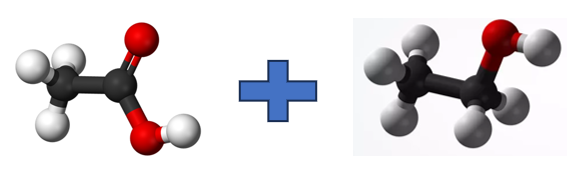
\includegraphics[width=0.86\linewidth]{rasmlar/m_efir.png}\end{center}

\noindent\begin{tabular}{@{}p{0.47\linewidth}@{}p{0.47\linewidth}@{}}
A)~\textsl{metilatsetat} & B)~\textsl{etilformiat} \\
C)~\textsl{etilatsetat} & D)~\textsl{propil spirti} \\
\end{tabular}\par
\qsep
\noindent\qn{24.} Anilin va metilamin aralashmasi (10,85 g) mo`l bromli suv bilan ta'sirlashganda 16,5 g cho`kma tushdi. Aralashmadagi metilaminning \textbf{massasini (g) toping.}

\noindent A)~\textsl{6,2} \hfill B)~\textsl{4,65} \hfill C)~\textsl{12,4} \hfill D)~\textsl{5,43}\par
\qsep
\noindent\qn{25.} Butan qizdirilib, quyidagi sxema bo`yicha parchalandi: C\textsubscript{4}H\textsubscript{10} $\to$ C\textsubscript{2}H\textsubscript{6} + C\textsubscript{2}H\textsubscript{4}. Hosil bo`lgan gazlar aralashmasining vodorodga nisbatan zichligi 14,5 bo`lsa, butanning parchalanish \textbf{unumini (\%) aniqlang.}

\noindent A)~\textsl{100} \hfill B)~\textsl{50} \hfill C)~\textsl{80} \hfill D)~\textsl{200}\par
\qsep
\noindent\qn{26.} C\textsubscript{6}H\textsubscript{6} dan quyidagi sxema bo`yicha 167,04 g natriy fenolyat olindi: C\textsubscript{6}H\textsubscript{6} $\to$ C\textsubscript{6}H\textsubscript{5}Cl $\to$ C\textsubscript{6}H\textsubscript{5}OH $\to$ C\textsubscript{6}H\textsubscript{5}ONa. Bosqichlarning unumi ketma-ket 75\%, 80\%, 60\% ni tashkil qiladi. Sarflangan C\textsubscript{6}H\textsubscript{6} massasi (g) \textbf{ni aniqlang.}

\noindent A)~\textsl{624} \hfill B)~\textsl{156} \hfill C)~\textsl{234} \hfill D)~\textsl{312}\par
\qsep
\noindent\qn{27.} Chumoli va sirka kislota aralashmasi mo`l NaHCO\textsubscript{3} eritmasi bilan ta'sirlashganda 11,2 l (n.sh.) gaz ajraldi. Shu miqdordagi aralashma ammiakli kumush oksid bilan qizdirilganda 21,6 g kumush hosil bo`ldi. Qizdirish 30 daqiqa davom etdi. Aralashmadagi sirka kislotaning \textbf{massasini (g) toping.}

\noindent A)~\textsl{4,6} \hfill B)~\textsl{24} \hfill C)~\textsl{48} \hfill D)~\textsl{12}\par
\qsep
\noindent\qn{28.} 312 g C\textsubscript{6}H\textsubscript{6} dan quyidagi sxema bo`yicha 381,31 g 2,4,6-tribromfenol olindi: C\textsubscript{6}H\textsubscript{6} $\to$ C\textsubscript{6}H\textsubscript{5}Cl $\to$ C\textsubscript{6}H\textsubscript{5}OH $\to$ C\textsubscript{6}H\textsubscript{2}Br\textsubscript{3}OH. Dastlabki 2 bosqichning unumi ketma-ket 90\%, 40\% ga teng. Barcha reaksiyalar 2 atm bosimda olib borildi. Oxirgi bosqichning \textbf{unumini (\%) aniqlang.}

\noindent A)~\textsl{40} \hfill B)~\textsl{20} \hfill C)~\textsl{80} \hfill D)~\textsl{64}\par
\qsep
\noindent\qn{29.} 44,8 l (n.sh.) CH\textsubscript{4} dan quyidagi sxema bo`yicha formaldegid olindi: CH\textsubscript{4} $\to$ CH\textsubscript{3}Cl $\to$ CH\textsubscript{3}OH $\to$ HCHO. Bosqichlarning unumi ketma-ket 85\%, 40\%, 80\% ni tashkil qiladi. Olingan formaldegid \textbf{massasini (g) aniqlang.}

\noindent A)~\textsl{32,64} \hfill B)~\textsl{8,16} \hfill C)~\textsl{16,32} \hfill D)~\textsl{20,4}\par
\qsep
\noindent\qn{30.} Temir(II) xlorid va temir(III) xlorid eritmalarini (moddalarini) bir-biridan qaysi reagent yordamida farqlash mumkin?

\noindent\begin{tabular}{@{}p{0.47\linewidth}@{}p{0.47\linewidth}@{}}
A)~\textsl{xlorid kislota} & B)~\textsl{kaliy rodanid (KSCN)} \\
C)~\textsl{bariy xlorid} & D)~\textsl{kumush nitrat} \\
\end{tabular}\par
\qsep
\noindent\qn{31.} Laboratoriyada olingan asetilen qanday usulda yig`iladi?
\noindent A)~\textsl{ochiq havoda tutib olinadi}\par
\noindent B)~\textsl{gazni suyuqlantirib yig`iladi}\par
\noindent C)~\textsl{suvni siqib chiqarish usulida}\par
\noindent D)~\textsl{havoni siqib chiqarish (idish og`zi pastga)}\par
\qsep
\noindent\qn{32.} Rasmdagi usul bilan qaysi moddani eritmadan ajratib olish mumkin?
\begin{center}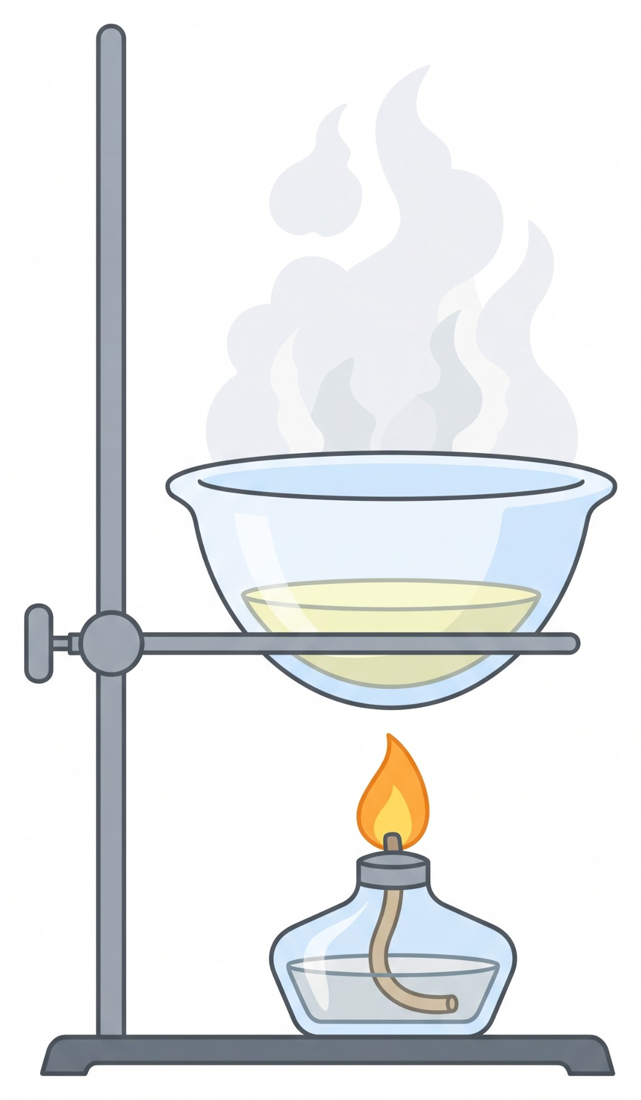
\includegraphics[width=0.86\linewidth]{rasmlar/darslik/d_bugla.png}\end{center}
\noindent A)~\textsl{suvni osh tuzi eritmasidan (toza holda)}\par
\noindent B)~\textsl{qumni suvdan}\par
\noindent C)~\textsl{kerosinni suvdan}\par
\noindent D)~\textsl{osh tuzini tuz eritmasidan   ---}\par
\qsep
\end{multicols}
\medskip
\noindent\setlength{\fboxsep}{0pt}\fbox{\begin{tabular}{p{0.74\linewidth}|p{0.2\linewidth}}
\parbox[t]{0.72\linewidth}{\vspace{3pt}\textbf{Topshiriqlar (33--35) va javob variant (A--F)larini o`zaro to`g`ri moslashtiring.} 2 mol ammiakning yarmi nitrat kislotagacha qayta ishlandi (jami unum 100\%), qolgan ammiak hosil bo`lgan kislota bilan neytrallandi.
\vspace{3pt}} & \parbox[t]{0.19\linewidth}{\vspace{3pt}A~\textsl{80}\\[3pt]
B~\textsl{31,5}\\[3pt]
C~\textsl{63}\\[3pt]
D~\textsl{22,4}\\[3pt]
E~\textsl{44,8}\\[3pt]
F~\textsl{17,92}}\\ \hline
\parbox[t]{0.72\linewidth}{\vspace{2pt}\textbf{33. Hosil bo`lgan nitrat kislota massasini (g) aniqlang.}\vspace{2pt}} & \\ \hline
\parbox[t]{0.72\linewidth}{\vspace{2pt}\textbf{34. Neytrallanishda hosil bo`lgan ammoniy nitrat massasini (g) toping.}\vspace{2pt}} & \\ \hline
\parbox[t]{0.72\linewidth}{\vspace{2pt}\textbf{35. Qolgan ammiakning n.sh. dagi hajmini (l) hisoblang (neytrallashgacha).}\vspace{2pt}} & 
\end{tabular}}
\par\bigskip
\noindent\qn{36.} Mg + H\textsubscript{2}SO\textsubscript{4} $\to$ MgSO\textsubscript{4} + H\textsubscript{2}S + H\textsubscript{2}O reaksiya tenglamasini tenglang va barcha koeffitsiyentlar \textbf{yig`indisini aniqlang.}
\javob\qsep
\noindent\qn{37.} CO + H\textsubscript{2}O $\rightleftarrows$ CO\textsubscript{2} + H\textsubscript{2} sistemasida boshlang`ich moddalarning har biridan 4 mol dan 1 l hajmli idishga solindi. Muvozanat qaror topganda reagentlarning har birining 3/5 qismi sarflangan bo`ldi. Tajriba 10 daqiqa davom etdi. Muvozanat \textbf{konstantasini hisoblang.}
\javob\qsep
\noindent\qn{38.} Oksidlanish darajasi +3 bo`lgan noma'lum \textit{X} metallning xloridi 7,93 g massada mo`l AgNO\textsubscript{3} eritmasi bilan ta'sirlashganda 21,53 g cho`kma hosil bo`ldi. Reagent (AgNO\textsubscript{3}) eritmasining massa ulushi 10\% va zichligi 1,12 g/ml; u mo`l miqdorda olingan. \textit{X} metallning nisbiy atom \textbf{massasini toping.}
\javob\qsep
\noindent\qn{39.} 11,2 l (n.sh.) atsetilen Kucherov reaksiyasi bo`yicha gidratlandi (unum 1/2); hosil bo`lgan aldegidning 1/2 qismi ammiakli kumush oksid eritmasi bilan qizdirildi. Ajralgan kumush \textbf{massasini (g) hisoblang.}
\javob\qsep
\noindent\qn{40.} Bir asosli to`yingan karbon kislotaning 52,8 g miqdori mo`l NaHCO\textsubscript{3} bilan ta'sirlashganda 13,44 l (n.sh.) gaz ajraldi. Shu kislotaning 2/3 qismi mo`l etanol bilan esterlandi (efir unumi 4/5). Barcha reaksiyalar 2 atm bosimda olib borildi. Hosil bo`lgan murakkab efirning \textbf{massasini (g) toping.}
\javob\qsep
\par\bigskip\begin{center}\textbf{\fontsize{13}{15}\selectfont YOZMA ISH}\end{center}
\noindent\qn{41.} \textbf{Topshiriqni bajarish jarayonida barcha reaksiya tenglamalarini yozing. Miqdoriy va arifmetik hisoblashlarni (unga asos bo`lgan usul yoki formulani ko`rsatgan holda) uzviy ketma-ketlikda bajaring.}\par\smallskip
47,4 g KMnO\textsubscript{4} qizdirilganda qisman parchalandi. Ajralgan kislorodning hajmi 27 \textdegree{}C va 83,14 kPa da 2,7 l ga teng bo`ldi (R = 8,314 J/(mol$\cdot$K)). Qattiq qoldiq mo`l konsentrlangan xlorid kislota bilan qizdirildi (K\textsubscript{2}MnO\textsubscript{4}, MnO\textsubscript{2} va parchalanmay qolgan KMnO\textsubscript{4} ning barchasi reaksiyaga kirishdi).\par
\noindent 1)\ Parchalanish va qattiq qoldiqning xlorid kislota bilan reaksiyalarini yozing va tenglashtiring (elektron balans).\par
\noindent 2)\ KMnO\textsubscript{4} ning necha foizi parchalanganini aniqlang.\par
\noindent 3)\ Qattiq qoldiq massasini (g) va undagi MnO\textsubscript{2} ning massa ulushini (\%) toping.\par
\noindent 4)\ Ajralgan xlorning umumiy hajmini (l, n.sh.) va sarflangan HCl miqdorini (mol) hisoblang.\par
\noindent 5)\ Reaksiyadan so`ng eritmadagi tuzlarning (KCl va MnCl\textsubscript{2}) umumiy massasini (g) toping.\par
\diqqat{Mazkur topshiriq kengaytirilgan javobni talab etib, uning yechilish usuli va shu usul asosidagi barcha hisoblash amallari javoblar varaqasida aks etishi lozim.}\qsep
\noindent\qn{42.} Quyidagi o`zgarishlar zanjirida \textit{X}, \textit{Y}, \textit{Z} noma'lum organik moddalar:\par
\[\setlength{\fboxsep}{0pt}\text{CH\textsubscript{3}Cl}\xrightarrow{\text{Na}}\text{\textit{X}}\xrightarrow{\text{Cl\textsubscript{2}, yorug`lik}}\text{\textit{Y}}\xrightarrow{\text{KOH (spirtli)}}\text{C\textsubscript{2}H\textsubscript{4}}\]
\noindent 1)\ CH\textsubscript{3}Cl $\to$ \textit{X} : reaksiya tenglamasini yozing; hosil bo`lgan moddani nomlang.\par
\noindent 2)\ \textit{X} $\to$ \textit{Y} : reaksiya tenglamasini yozing; hosil bo`lgan moddani nomlang.\par
\noindent 3)\ \textit{Y} $\to$ C\textsubscript{2}H\textsubscript{4} : reaksiya tenglamasini yozing; hosil bo`lgan moddani nomlang.\par
\diqqat{Mazkur topshiriq kengaytirilgan javobni talab etib, uning yechilish usuli va shu usul asosidagi barcha hisoblash amallari javoblar varaqasida aks etishi lozim.}\qsep
\noindent\qn{43.} \textbf{Topshiriqni bajarish jarayonida barcha reaksiya tenglamalarini yozing. Miqdoriy va arifmetik hisoblashlarni (unga asos bo`lgan usul yoki formulani ko`rsatgan holda) uzviy ketma-ketlikda bajaring.}\par\smallskip
NO\textsubscript{2} va O\textsubscript{2} aralashmasi (27 \textdegree{}C, 83,14 kPa da hajmi 33 l) 300 g suvga yuborildi. Yutilmay qolgan gaz hajmi shu sharoitda 3 l bo`ldi. R = 8,314 J/(mol$\cdot$K). Olingan nitrat kislota eritmasiga stexiometrik miqdorda CaCO\textsubscript{3} qo`shildi, hosil bo`lgan tuz eritmasi bug`latilib, qoldiq doimiy massagacha qizdirildi, ajralgan gazlar suvga yuttirildi.\par
\noindent 1)\ Reaksiya tenglamalarini yozing va qaysi gaz ortiqcha bo`lganini aniqlang.\par
\noindent 2)\ Dastlabki aralashmadagi NO\textsubscript{2} va O\textsubscript{2} ning mol miqdorlarini hamda hajmiy ulushlarini (\%) toping.\par
\noindent 3)\ Hosil bo`lgan eritmadagi HNO\textsubscript{3} ning massasini (g) va massa ulushini (\%) hisoblang. Kislotani neytrallash uchun sarflangan CaCO\textsubscript{3} massasini (g) va ajralgan CO\textsubscript{2} hajmini (l, n.sh.) toping.\par
\noindent 4)\ Dastlabki aralashmadagi NO\textsubscript{2} va O\textsubscript{2} ning massalarini (g) toping. Bug`latib qizdirilgandan keyin qolgan qattiq moddaning massasini (g) hisoblang.\par
\noindent 5)\ Dastlabki aralashmaning havoga nisbatan zichligini (M(havo) = 29 g/mol) aniqlang. Ajralgan gazlar suvga yuttirilganda qayta hosil bo`lgan HNO\textsubscript{3} massasini (g) aniqlang.\par
\diqqat{Mazkur topshiriq kengaytirilgan javobni talab etib, uning yechilish usuli va shu usul asosidagi barcha hisoblash amallari javoblar varaqasida aks etishi lozim.}\qsep
\newpage
\noindent\textbf{\fontsize{13}{15}\selectfont 11-variant}\hfill \textbf{Javoblar kaliti}\par\smallskip\hrule\smallskip
\textit{Faqat o`qituvchi uchun.}\par\medskip
\noindent\textbf{1--32-savollar}\par\smallskip
\noindent\begin{tabular}{|c|c|c|c|c|c|c|c|c|c|c|c|c|c|c|c|}\hline
\textbf{1} & \textbf{2} & \textbf{3} & \textbf{4} & \textbf{5} & \textbf{6} & \textbf{7} & \textbf{8} & \textbf{9} & \textbf{10} & \textbf{11} & \textbf{12} & \textbf{13} & \textbf{14} & \textbf{15} & \textbf{16}\\\hline
\textsl{C} & \textsl{D} & \textsl{A} & \textsl{D} & \textsl{A} & \textsl{B} & \textsl{D} & \textsl{D} & \textsl{B} & \textsl{C} & \textsl{A} & \textsl{D} & \textsl{A} & \textsl{B} & \textsl{C} & \textsl{B}\\\hline
\textbf{17} & \textbf{18} & \textbf{19} & \textbf{20} & \textbf{21} & \textbf{22} & \textbf{23} & \textbf{24} & \textbf{25} & \textbf{26} & \textbf{27} & \textbf{28} & \textbf{29} & \textbf{30} & \textbf{31} & \textbf{32}\\\hline
\textsl{B} & \textsl{A} & \textsl{A} & \textsl{D} & \textsl{C} & \textsl{B} & \textsl{C} & \textsl{A} & \textsl{A} & \textsl{D} & \textsl{B} & \textsl{C} & \textsl{C} & \textsl{B} & \textsl{C} & \textsl{D}\\\hline
\end{tabular}\par\medskip
\noindent\textbf{33--35-savollar}\par\smallskip
\noindent\begin{tabular}{|c|c|c|}\hline \textbf{No} & \textbf{Javob} & \textbf{Qiymat}\\\hline
33 & \textsl{C} & 63\\\hline
34 & \textsl{A} & 80\\\hline
35 & \textsl{D} & 22,4\\\hline
\end{tabular}\par\medskip
\noindent\textbf{36--40-savollar}\par\smallskip
\noindent\begin{tabular}{|c|c|}\hline \textbf{No} & \textbf{To`g`ri javob}\\\hline
36 & 18\\\hline
37 & 2,25\\\hline
38 & 52\\\hline
39 & 27\\\hline
40 & 37,12\\\hline
\end{tabular}\par\medskip
\noindent\textbf{41--43-topshiriqlar: javoblar}\par\smallskip
\noindent\textbf{41-topshiriq.}\par
\noindent 1) 2KMnO\textsubscript{4} $\to$ K\textsubscript{2}MnO\textsubscript{4} + MnO\textsubscript{2} + O\textsubscript{2}$\uparrow$; K\textsubscript{2}MnO\textsubscript{4} + 8HCl $\to$ 2KCl + MnCl\textsubscript{2} + 2Cl\textsubscript{2} + 4H\textsubscript{2}O; MnO\textsubscript{2} + 4HCl $\to$ MnCl\textsubscript{2} + Cl\textsubscript{2} + 2H\textsubscript{2}O; 2KMnO\textsubscript{4} + 16H\par
\noindent 2) 60\%\par
\noindent 3) 44,52 g; 17,6\%\par
\noindent 4) 12,77 l; 2,04 mol\par
\noindent 5) 60,15 g\par
\noindent\textbf{42-topshiriq.}\par
\noindent 1) CH\textsubscript{3}Cl + Na $\to$ C\textsubscript{2}H\textsubscript{6} (etan)\par
\noindent 2) C\textsubscript{2}H\textsubscript{6} + Cl\textsubscript{2}, yorug`lik $\to$ C\textsubscript{2}H\textsubscript{5}Cl (xloretan)\par
\noindent 3) C\textsubscript{2}H\textsubscript{5}Cl + KOH (spirtli) $\to$ C\textsubscript{2}H\textsubscript{4} (etilen)\par
\noindent\textbf{43-topshiriq.}\par
\noindent 1) O\textsubscript{2}\par
\noindent 2) 0,8 mol; 0,3 mol\par
\noindent 3) 14,69\%; 40 g; 8,96 l\par
\noindent 4) 36,8 g; 9,6 g; 22,4 g\par
\noindent 5) 1,45; 50,4 g\par
\par\bigskip\noindent\textbf{Mavzular taqsimoti}\par\smallskip
{\small\noindent\begin{longtable}{|c|p{7.2cm}|p{5.4cm}|c|}\hline \textbf{No} & \textbf{Mavzu} & \textbf{Tekshiriladigan ko`nikma} & \textbf{Ball}\\\hline
1 & 7-sinf (jism va modda) & Bilim va tushunish & 1\\\hline
2 & 11-sinf 8-bob; Tirkashev \textit{V} bob (elektroliz) & Bilim va tushunish & 1\\\hline
3 & 8-sinf (izotoplar, izobarlar, jadval) & Jadval tahlili & 1\\\hline
4 & 9-sinf; 10-sinf (tuzlar gidrolizi, ion almashinish reaksiyalari) & Bilim va tushunish & 1\\\hline
5 & 8-sinf; Tirkashev II bob (kimyoviy bog`lanish) & Bilim va tushunish & 1\\\hline
6 & Tirkashev I bob (kvant sonlari) & Bilim va tushunish & 1\\\hline
7 & 7-sinf (valentlik) & Bilim va tushunish & 1\\\hline
8 & 11-sinf (radioaktivlik; yarim yemirilish davri) & Hisoblash va masala yechish & 1\\\hline
9 & 8-sinf (ionlanish energiyasi, grafik) & Grafik tahlili & 1\\\hline
10 & 8-sinf (ortiqcha modda masalasi) & Hisoblash va masala yechish & 1\\\hline
11 & Tirkashev III bob (eritmalar, jadval) & Jadval tahlili & 1\\\hline
12 & Tirkashev III bob (eritmalar, jadval) & Jadval tahlili & 1\\\hline
13 & 9-11-sinf (kimyoviy muvozanat) & Hisoblash va masala yechish & 1\\\hline
14 & Tashev (nodir gazlar); 8-sinf & Bilim va tushunish & 1\\\hline
15 & Tashev (nitratlar) & Bilim va tushunish & 1\\\hline
16 & 9-sinf (nitratlarning termik parchalanishi) & Hisoblash va masala yechish & 1\\\hline
17 & 9-sinf (ko`p negizli kislotalar, nordon tuzlar) & Hisoblash va masala yechish & 1\\\hline
18 & 9-sinf (xloridlar; sifat reaksiyasi) & Hisoblash va masala yechish & 1\\\hline
19 & Tashev (H\textsubscript{2}SO\textsubscript{4} olinishi) & Hisoblash va masala yechish & 1\\\hline
20 & 10-sinf (olinish usullari) & Bilim va tushunish & 1\\\hline
21 & 10-sinf (spirt, aldegid, fenol sifat reaksiyalari) & Bilim va tushunish & 1\\\hline
22 & 10-sinf (alkinlar, aldegidlar, karbon kislotalar) & Hisoblash va masala yechish & 1\\\hline
23 & 10-sinf \S{}28 & Rasm bo`yicha tahlil & 1\\\hline
24 & 10-sinf (aminlar va anilin xossalari) & Hisoblash va masala yechish & 1\\\hline
25 & 10-sinf (alkanlarning krekingi va degidrogenlanishi) & Hisoblash va masala yechish & 1\\\hline
26 & 10-sinf (arenlar, fenol) & Hisoblash va masala yechish & 1\\\hline
27 & 10-sinf (karbon kislotalar; chumoli kislotaning o`ziga xosligi) & Hisoblash va masala yechish & 1\\\hline
28 & 10-sinf (arenlar, fenol) & Hisoblash va masala yechish & 1\\\hline
29 & 10-sinf (galogenlash, gidroliz, spirtning oksidlanishi) & Hisoblash va masala yechish & 1\\\hline
30 & 9-sinf; 10-sinf (sifat reaksiyalari; moddalarni farqlash) & Bilim va tushunish & 1\\\hline
31 & 9--10-sinf (gazlarni yig`ish) & Bilim va tushunish & 1\\\hline
32 & 7-sinf (12-rasm) & Rasm bo`yicha tahlil & 1\\\hline
33--35 & Aralash masala (moslashtirish) & Ko`p bosqichli hisob & 3\\\hline
36--40 & Qisqa javobli masalalar & Hisoblash & 5\\\hline
41--43 & Yozma ish & Usul va hisob (M, A) & 75\\\hline
\end{longtable}}
\end{document}
